\section{Vzorkovací obvody}
- S/H a T/H obvody - rozdíly, funkce, základní parametry, příklady realizací
\subsection{S/H a T/H obvody}
\textbf{Vzorkovač s pamětí – S/H (sample and hold)}, který sejme v daném okamžiku vzorek signálu a podrží si jeho hodnotu, při příchodu dalšího řídicího pulzu uloží novou, aktuální hodnotu.

\textbf{Sledovač s pamětí – T/H (track and hold)}, sleduje (kopíruje) průběh signálu a ukládá si aktuální hodnotu až s příchodem řídicího impulzu.

\subsection{Funkce}

\subsection{Základní parametry}
\textbf{Zesílení (gain)} je střední strmost statické převodní charakteristiky. Udává se možná
chyba zesílení a rozsah seřizovacích možností.

\textbf{Vstupní napěťový rozsah (input voltage range)} je povolené napětí, při kterém platí
jmenovité parametry.

\textbf{Výstupní napěťový rozsah (output voltage range)} je rozsah výstupního napětí, kdy ještě
nedochází k omezení výstupního napětí.

\textbf{Vstupní napěťová nesymetrie (input voltage offset)} je vstupní napětí, při kterém je
výstupní právě rovno nule

\textbf{Nelinearita (linearity)} udává maximální odchylku výstupního napětí od jmenovité hodnoty. Měří se po přesném nastavení zesílení a vynulování offsetu, udává se většinou v \%.

\textbf{Činitel potlačení vstupního napětí (feedthrough rejection ratio)} udává převrácenou
hodnotu přenosu vstupního napětí na výstup v paměťovém provozu. Někdy se udává
v závislosti na kapacitě paměťového kapacitoru. Jednotkou obvykle bývá dB.

\textbf{Rychlost klesání výstupního napětí (droop rate)} je změna výstupního napětí za jednotku
času po zapamatování napětí. Je způsobeno svodovými proudy paměťového kapacitoru a
klidovými proudy připojených obvodů. Obvykle se udává v závislosti na kapacitě
paměťového kapacitoru.
   \begin{figure}[h]
   \begin{center}
     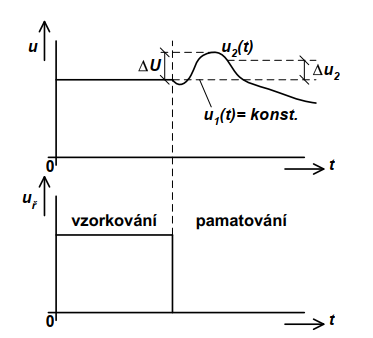
\includegraphics[scale=0.6]{images/Droop.png}
   \end{center}
   \caption{Skutečný průběh pamatování ve vzorkovači}
  \end{figure}
\pagebreak

\subsubsection{Základní parametry související s přechodovými ději}
\textbf{Doba upnutí (acquisition time)} je doba potřebná k přechodu z paměťového do sledovacího provozu. Definuje se pro udaný skok výstupního napětí (nejhorší je skok přes celé rozmezí povoleného výstupního napětí) s následným ustálením v předepsaném tolerančním pásu při ss nebo pomalu se měnícím vstupním napětí

\textbf{Rychlost přeběhu (slew rate)} je maximální rychlost změny výstupního napětí. U provedení s vnějším C\textsubscript{p} se udává v závislosti na tomto kapacitoru nebo se udává maximální nabíjecí proud I\textsubscript{max} (buď konečný proud, který je schopen dodat předřazený OZ nebo proud, který může téct maximálně spínačem – volí se ten, který je menší). Uvažují-li se neomezené proudové schopnosti zdroje vstupního signálu, pak se při vzorkování C\textsubscript{p} nabíjí přes sériovou kombinaci nenulového vnitřního odporu zdroje vstupního signálu R\textsubscript{i} a odporu sepnutého spínače R\textsubscript{sep} s časovou konstantou:
\begin{equation}
\tau = (R_{i}+R_{sep}*C_{p})
\end{equation}

Doba vzorkování nutná pro dosažení dané přesnosti
\begin{itemize}
\item pro přesnost 10\%: 
\begin{equation}
\tau \geq 3*(R_{i}+R_{sep}*C_{p})
\end{equation}
\item pro přesnost 1\%: 
\begin{equation}
\tau \geq 5*(R_{i}+R_{sep}*C_{p})
\end{equation}
\item pro přesnost 0,1\%: 
\begin{equation}
\tau \geq 7*(R_{i}+R_{sep}*C_{p})
\end{equation}
\item pro přesnost 0,01\%: 
\begin{equation}
\tau \geq 9*(R_{i}+R_{sep}*C_{p})
\end{equation}
\end{itemize}

\textbf{Doba ustálení (settling time)} je doba potřebná k přechodu ze vzorkovacího do ustáleného paměťového režimu. Měří se doba ustálení signálu v daném tolerančním pásmu.

\textbf{Přepínací skokové napětí (sample-to-hold offset)} je chyba sejmutí vzorku v důsledku
průniku řidicího signálu přes parazitní kapacity spínače. V provedení s vnějším C\textsubscript{p} se uvede
velikost náboje přeneseného na C\textsubscript{p}.

\textbf{Apertura (časová neurčitost – aperture)} je způsobena reálnými vlastnostmi těch částí
vzorkovače, které realizují přechod obvodu z režimu vzorkování do pamatování.

\textbf{Efektivní okamžik sejmutí vzorku (effective sampling time) t\textsubscript{ef}} je okamžik, v němž by
měl monotónně se měnící vstupní signál velikost, na které se ustálí napětí na C\textsubscript{p}.

\textbf{Doba apertury (aperture time)} je doba mezi bezprostředním pokynem k rozpojení
spínače a ukončením rozpojování, kdy lze spínač považovat za zcela rozpojený.

\textbf{Nejistota apertury (aperture uncertainty)} je náhodné kolísání doby apertury. Někdy se
označuje jako aperturové chvění (jitter).

\textbf{Fázové zpoždění (phase delay)} je doba mezi bezprostředním podnětem k rozpojení
spínače a \textsubscript{ef}.

\textbf{Aperturová chyba (aperture error)} je nepřesnost sejmutí vzorku v důsledku aperturového
chvění a s kmitočtem roste
   \begin{figure}[h]
   \begin{center}
     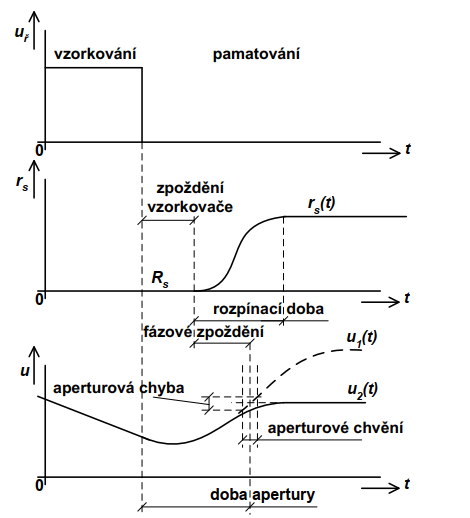
\includegraphics[scale=0.6]{images/Apertura.png}
   \end{center}
   \caption{Apertura}
  \end{figure}
  
\textbf{Zpoždění vzorkovače (S/H delay, T/H delay)} je doba mezi příkazem k sejmutí vzorku a bezprostředním podnětem k rozpojení spínače.

\subsection{Příklady realizací}
Realizace vzorkovače je v drtivé většině případů řešena zapojením v technice SC. V současné době se však dostává do popředí zájmu i technika spínaných proudů (SI) a to zejména díky pracovnímu režimu, který je proudový, čehož je využíváno ke snižování napájecích napětí.







